\chapter{Approach}
\label{chap:approach}
This chapter introduces the distinctive concept of a configurable search engine and outlines the comprehensive software architecture. It thoroughly explores and showcases all the required components for constructing the search engine, along with discussing implementation specifics. This encompasses the pivotal models and classes employed for the components and algorithms.
Furthermore, the chapter delves into the user interface, clarifying how it enhances user experience and facilitates configuring the search engine.

\section{Software Architecture}

Figure 4 provides an overview of the software architecture employed by the search engine. Microservices architecture was used to make scalability easier and also to split the responsibilities of each component. Docker is used to enforce this architectural pattern where the Ubuntu:18.04 image is used for each component. Below is a compilation of the utilized technology stack:

\begin{figure}[h]	
     \centering
     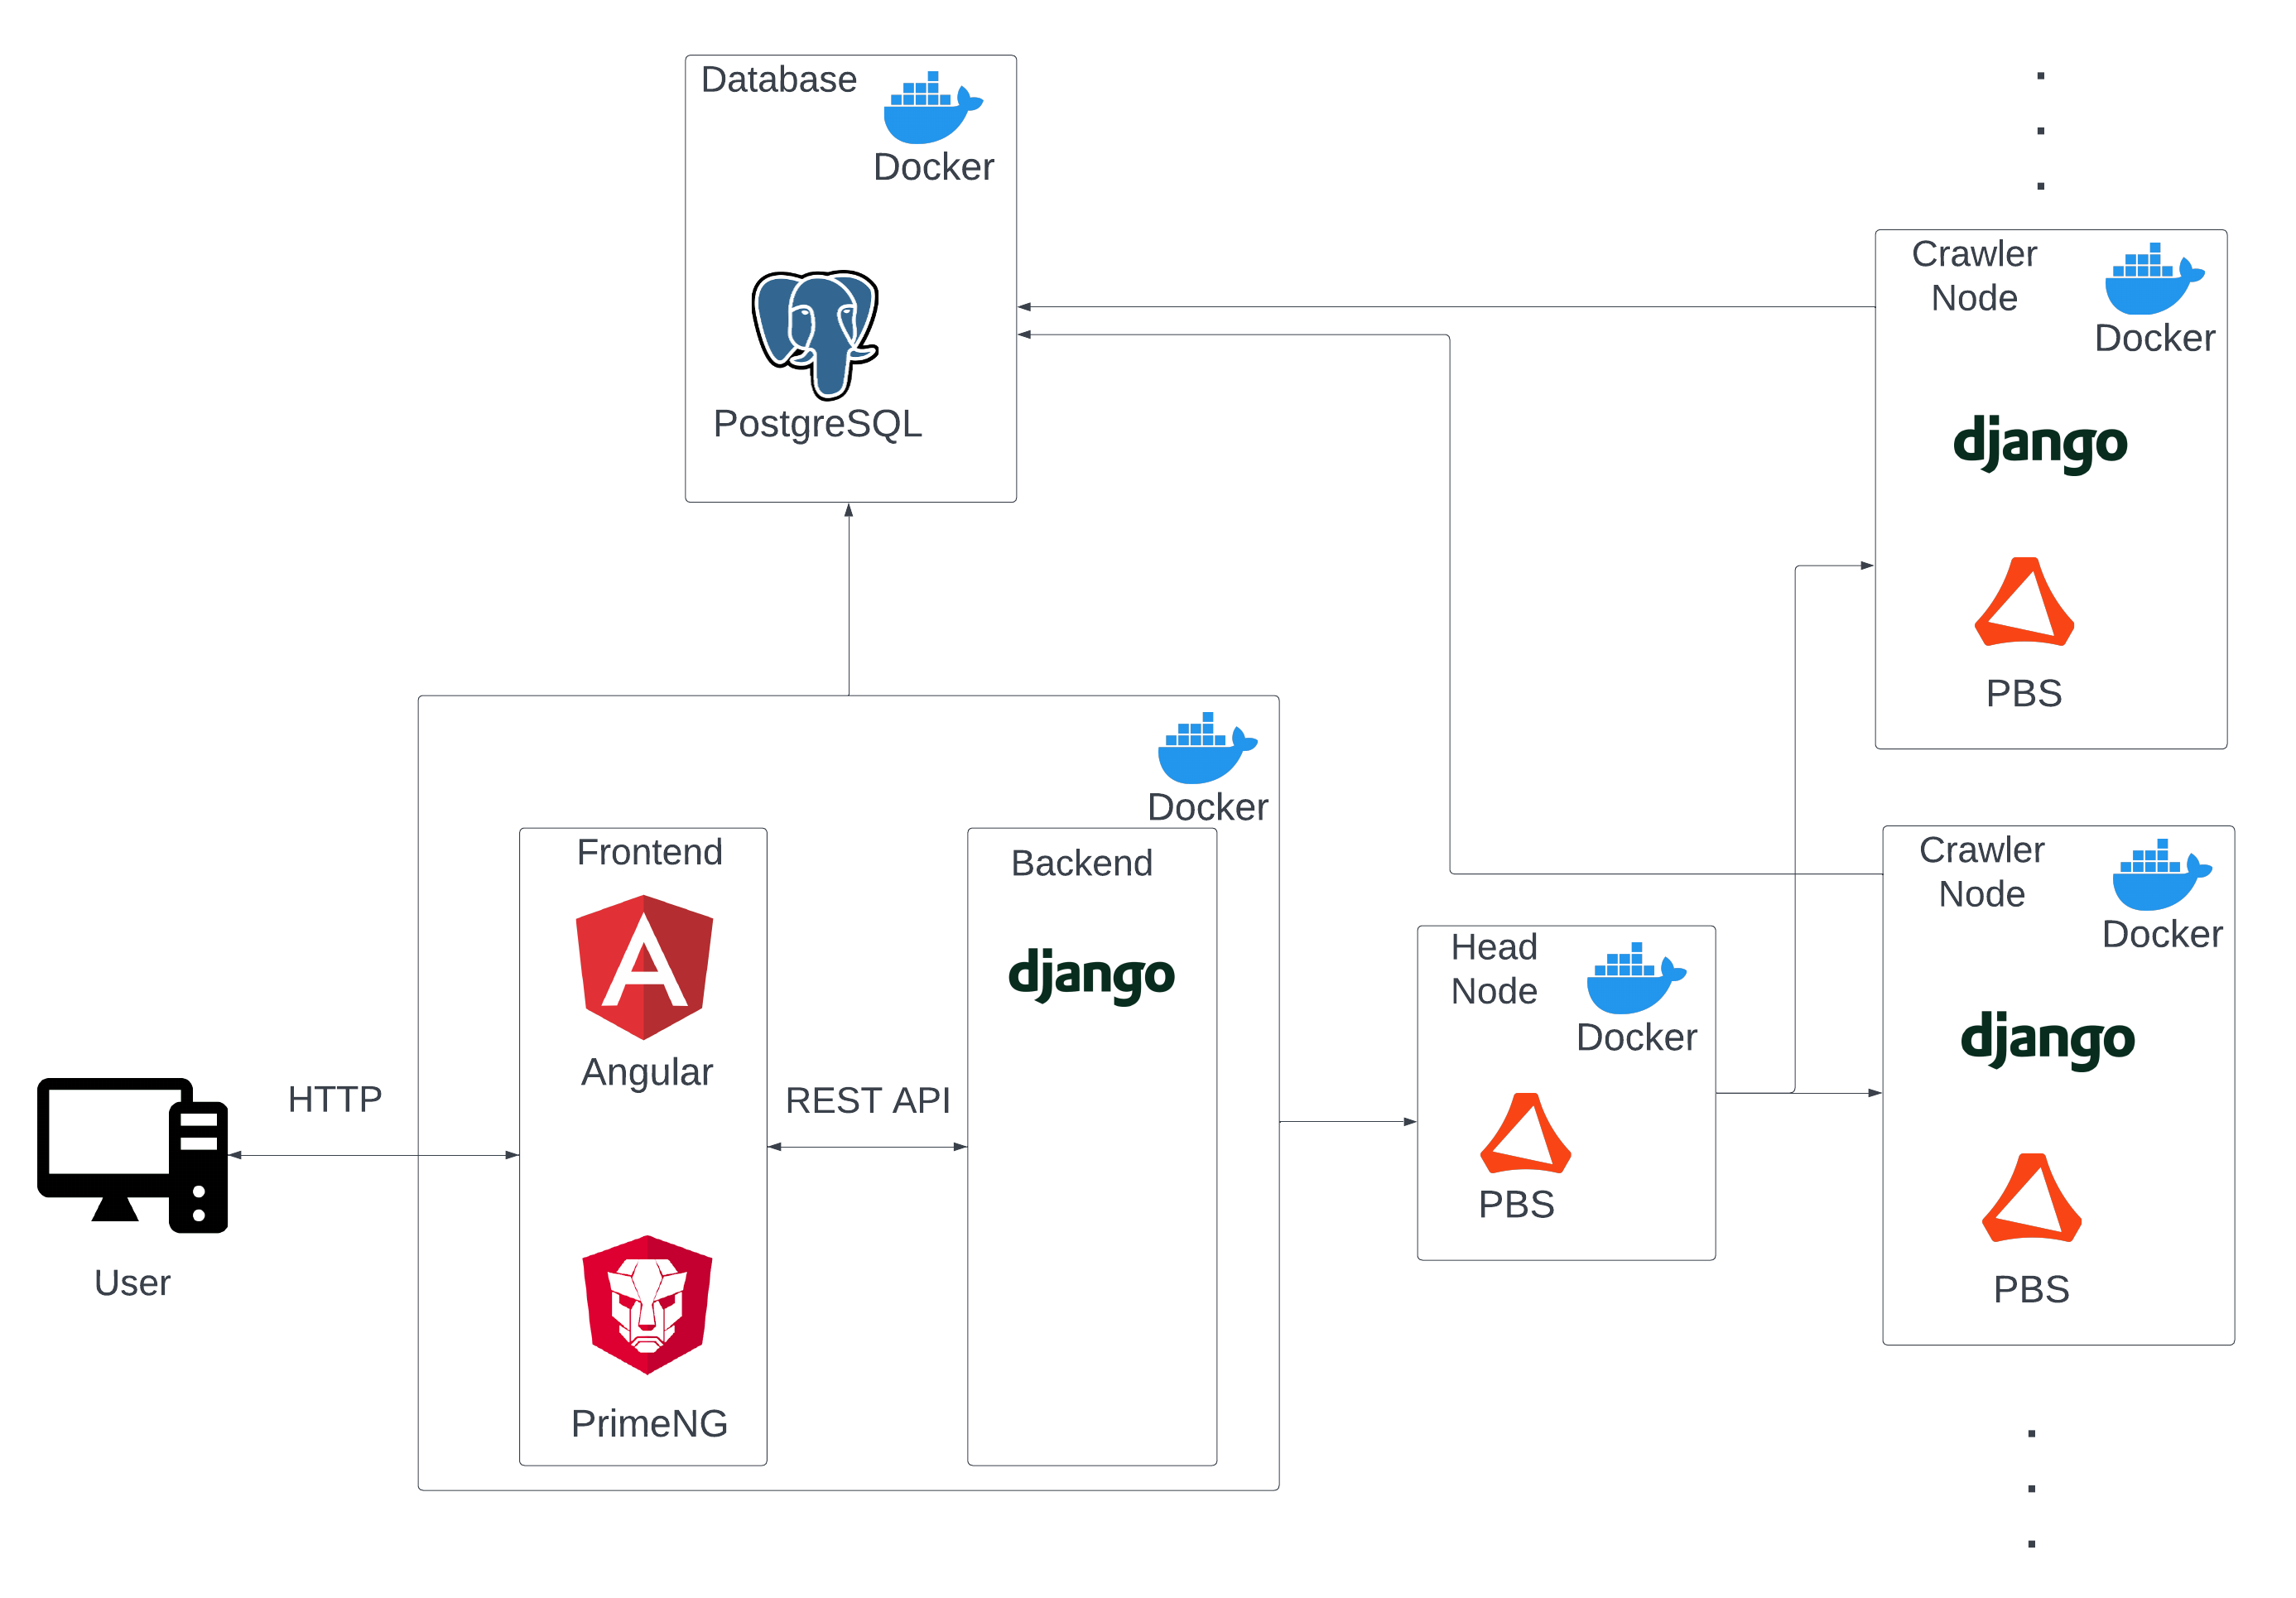
\includegraphics[width=10cm]{images/software_arch.png}
     \caption{High-level view of the software archtiticture.}
     \label{fig:software-arch}
\end{figure}

\begin{itemize}
  \item \textbf{Frontend (Angular \& PrimeNG)}: Positioned closest to the user, this component encompasses all pages and views. Angular is leveraged in conjunction with the contemporary CSS library, PrimeNG. To communicate with the backend, it employs the REST API.
  \item \textbf{Backend (Django)}: Serving as the core intelligence of the search engine, the backend houses both the crawler and indexer modules. It facilitates interaction with the Head node to initiate crawling based on user-defined configurations. Moreover, it establishes a connection with PostgreSQL for the storage of crawler and indexer configurations, along with job-related information.
  \item \textbf{Head Node (PBS)}: Operating as the central hub, this node orchestrates job management and determines the allocation of tasks to Crawler nodes, which are responsible for traversing the specified websites.
  \item \textbf{Crawler Node (PBS)}: These instances are designated to execute the crawling process and store the resulting data in the PostgreSQL database.
\end{itemize}

The application setup initiates with a minimal requirement of four microservices to operate the entire search engine. One Docker container containing both Angular and Backend logic must establish connections with two other containers: the Database and PBS Head Node. The PBS Head Node, in turn, should connect to one or more Crawler Node containers responsible for executing the crawling task. The Crawler Node will perform the crawling job and save the results to the shared Database.

The workflow begins with a user-friendly interface presented by Angular and PrimeNG, encompassing all the configurations and tools enabling users to crawl quickly and index various websites. Users can modify configurations and submit a crawling job to the Head Node. The Head Node, in response, identifies an available Crawler Node to execute the task. It's worth noting that the PBS cluster can be bypassed, and the crawling process can be run locally on a localhost server. Users can monitor the progress of the running job from the browser. Once crawling is completed and the user is happy with the result, the user can start indexing. The indexing job also does not support a distributed architecture and will be executed locally and not on the PBS cluster.


\section{Crawler Implmentation}

PBS Crawler Node runs the crawling job or can also run locally. The job supports multithreading. As illustrated by the pseudo-code shown in Algorithm [1], the crawler starts by loading the configuration submitted by the user from the Database. More details about the configuration are in the user interface section. Based on the configuration of a thread pool, the number of threads is read by the configuration. The thread pool contains all the threads crawling the site, where each thread contains a queue of URLs that it crawls from. The thread pool makes sure that if one thread has no URLs anymore, it can ask other threads to help. Algorithm [2] explains how this sharing URLs mechanism works. 


\begin{algorithm}[H]
	\caption{Start Crawling}\label{alg:alg1}
	\begin{algorithmic}[1]
		\State load\_crawler\_configurations()
		\State $thread$ $\gets$ create\_threads\_pool()
	    \State $urls\_queue$ $\gets$ get\_thread\_urls\_queue($thread)$)
	    \State $seed\_url$ $\gets$ get\_seed\_url()
	    \State add\_url\_to\_queue($urls\_queue$, $seed\_url$)
	    \State $robot\_file$ $\gets$ get\_robot\_file\_content()
	    \While {$urls\_queue$ not empty or all threads not done}
		\If{$urls\_queue$ is empty}
		    \State $urls\_queue$ $\gets$ get\_thread\_urls\_queue($thread$)
		\Else
			\State $current\_url$ $\gets$ urls\_queue\_next\_url()
			\State filter\_unwanted\_urls($current\_url$)
			\State request\_page($current\_url$)
            \State execute\_automated\_actions()
			\State find\_next\_urls\_and\_add\_them\_to\_urls\_queue()
			\State $docs$ $\gets$ find\_and\_download\_targeted\_documents()
			\State filter\_unwanted\_documents($docs$)
		\EndIf
		\EndWhile

	\end{algorithmic}
\end{algorithm}


A seed URL is added to the current thread queue. The seed URL represents the starting point for the crawling, and the user configuration defines it. Using the sead url, the robots.txt content is downloaded once and can be reused for the rest of the crawling process.    

Each thread goes into an infinite loop that will continue to run either if the URLs queue still contains URLs to be fetched or at least one thread is still running. This guarantees that although one thread is running, it can be that that thread contains a lot of URLs that need help with crawling, and the free threads can share the load with it. If the thread queue is empty, it will ask the pool to find the next URLs to fetch. Otherwise, the first URL in the queue will be fetched, and a request using Selenium will be made. Afterwards, automated actions such as scrolling down, waiting and clicking defined by the user are executed. Those actions give the power to control the browser by the user to mimic real agent behaviour. The action chain will be discussed more in the User Interface section.  

After the page is rendered and the automated actions are executed, the next step is to collect the next URLs and add them to the URLs queue. The last step is to parse the documents needed from the page and filter the duplicated documents. 


\subsection{Links Data Structure}
The website's page navigation algorithm can be likened to a Level Order Traversal. The tree structure is established in the following manner: the seed URL acts as the tree's root node, representing level 0. After you explore the root page's content and gather its URLs, these URLs are assigned to the next level, level 1. Each page within level 1 is then visited, its contained URLs are collected, and these newly collected URLs are assigned to level 2. This process continues as you move deeper into the website until a maximum depth is reached, which is pre-defined by the user.
This algorithm offers an advantage in that it makes it straightforward to prioritize pages based on their respective levels. For instance, in some scenarios, pages closer to the initial seed URL may receive higher priority, potentially yielding better outcomes. In other cases, deeper pages within the structure may hold more significance than those closer to the seed URL. Choosing the proper algorithm is possible in the UI.

\subsection{Practical Challenges}
\begin{itemize}
  \item \textbf{Avoiding Loops}: Looping is when a web crawler repeatedly visits and requests the same web pages or URLs in a never-ending cycle, often resulting in excessive traffic to the same content. This is problematic as it wastes resources can also be inefficient, and can prevent the crawler from continuing. The first method to prevent looping is to record all the URLs visited and crawled. Before making a new request, we check if the URL is in this list. If it is, skip crawling it again to prevent loops. The second method is to use URL normalization. Normalize URLs by removing unnecessary components such as query parameters, fragments, or trailing slashes. This helps ensure that URLs with different representations (e.g., with and without a trailing slash) are treated as the same URL.


\item  \textbf{Duplicated Content}: While the same web crawler avoids revisiting identical URLs to prevent content duplication, it's important to note that identical content may exist in different URLs paths within the same website. For instance, a men's shoe might be accessible via various links like "/winter/shoes/", "/men/shoes/", or "/sales/shoes/". Relying solely on the URL as a unique identifier to prevent content duplication is not foolproof.
A more effective approach involves comparing the content itself with the database after parsing. Instead of a straightforward content check against the database, which can pose performance challenges, we employ a more efficient method. We generate a unique hash code using the SHA-1 hashing algorithm based on the content string intended for storage. This hash code is then stored in the database.
Before saving any new content, we can verify if the hash code already exists in the database. This method ensures content uniqueness, even when it appears under different URLs on the same site, without the computational overhead of directly comparing lengthy content strings in the database.

\item  \textbf{Dynamic Content}:Crawling dynamic websites presents a distinct set of challenges compared to static websites. Dynamic sites generate content on the client side through technologies like JavaScript, adding complexity to the task of accessing and extracting data. A primary concern lies in uncovering concealed content that necessitates user interaction. For instance, certain websites hide lengthy content portions, revealing them only upon clicking a "read more" button. Additionally, most websites implement lazy loading, fetching content on-demand via AJAX requests.
To address these challenges, Selenium establishes a genuine session and fully renders the webpage. This approach allows for emulating user interactions using action chains, which simulate actions such as waiting, scrolling, and clicking. More details regarding this can be found in the User Interface section.

\item  \textbf{Termination Conditions}: Crawlers can be brought to a halt by establishing specific criteria to ensure termination. The initial criterion involves defining a maximum depth, which restricts the number of page transitions to a single level. Additionally, monitoring and restricting the total count of visited pages and collected documents is possible. Another method is to employ a wall time measurement to monitor the crawler's runtime duration and trigger an abort if the crawler exceeds the expected time frame.

\item  \textbf{Avoiding DOS}: Increasing the number of requests and expanding the crawler's capacity by adding more threads or nodes may seem enticing to boost performance. However, this approach carries a significant risk of overwhelming the targeted servers, potentially resulting in Distributed Denial of Service (DDoS) or Denial of Service (DoS) attacks. Servers can perceive this surge in requests as an attack, which could lead to the crawler being blacklisted and subsequently banned.
To mitigate this risk, it's crucial to introduce a waiting period between each request made by the same crawler. Additionally, when using Selenium, a deliberate delay of at least one second or more is already integrated to allow for the complete rendering of web pages. Nevertheless, these precautions alone may not prevent users from adding more nodes and executing DDoS attacks. Consequently, it is strongly advisable to exercise cautious management by monitoring and regulating the number of threads and nodes. This approach demonstrates respect for the targeted servers and helps prevent overloading them.
\end{itemize}

\\

\section{Indexer Implmentation}

The indexing phase follows the crawling step, as it necessitates the downloading of documents. Unlike crawling, which can be computationally intensive, indexing is relatively lightweight. Hence, it is carried out on the localhost with multithreading support.
Algorithm [2] clarifies the indexing process. Firstly, the algorithm loads the user-defined indexing configurations. You can find more details about these configurations in the User Interface Design section. Subsequently, an empty inverted list is initialized. An inverted list is a data structure used to associate words or terms with the documents in which they appear. In Python, it can be implemented as a dictionary (Dict[str, list[int]]), where each word serves as a key, and the corresponding value is a list of document IDs containing that word.


\begin{algorithm}[H]
	\caption{Create Inverted List}\label{alg:alg1}
	\begin{algorithmic}[1]
	    \Require $documents$ not empty
		\State $config$ $\gets$ load\_indexer\_configurations()
		\State $inverted\_list$ $\gets$ init\_inverted\_list()
		\State $threshold$ $\gets$ get\_small\_words\_threshold($config$)
	    \State $stop\_list$ $\gets$ stop\_words\_list($config$)
        \For{$doc$ in $documents$}
          \State $doc\_length$ $\gets$ 0}
          \State $words$ $\gets$ tokenize($doc$)}
          \For{$word$ in $words$}
          	\State $doc\_length$ $\gets$ 0}
          	\If{$word$ > threshold and $word$ not in $stop\_list$}
		    	\State add\_word\_and\_doc\_id\_to\_inverted\_list($word$, $doc.id$)
		    	\State $doc\_length$ $\mathrel{+}=$ 1}
			\EndIf
          \EndFor
          \State add\_to\_doc\_lengths\_list($doc\_length$)
        \EndFor
        \State calculate\_bm25\_score($inverted\_list$)
        \State cache($inverted\_list$)

	\end{algorithmic}
\end{algorithm}

The user specifies three variables: "threshold" and "stop\_list," which are retrieved from the database. The "threshold" represents the minimum word length required for tokenization from a document. The "stop\_list" is a predefined list of terms that should be omitted from the indexing process.
The algorithm then iterates through all the documents, performing the following steps for each one:
Initializes the document length as a counter, initially set to zero.
Tokenizes the document to obtain a list of words.
Iterates through the word list, checking each word's length against the threshold and verifying if it is not in the stop\_list. If these conditions are met, the word is added to the inverted list, and the document length counter is incremented by one.


Once the inverted list is constructed, we calculate the MB25 score based on equation 3.4. Afterwards, it is saved into a cache for future retrieval and use.

\section{User Interface Design}
The core focus of this thesis extends beyond merely building and designing a search engine. It also encompasses the vital objective of enabling users to effortlessly configure and utilize it. In the forthcoming section, we will delve into the User Interface design, workflow, and the user-facing configurations.

The user begins their journey on the homepage, where they can access documentation explaining how to utilize the application. The application's workflow commences with the creation of templates, which serve as blueprints for specifying the document fields to be extracted from web pages. It is a prerequisite to establish a unique template for each page, although the same template can also be applied across different websites. These templates consist of components referred to as "inspectors," each comprising the following attributes:

\begin{itemize}
  \item \textbf{Name}: This denotes the inspector's identifier, such as "Price" or "Title."

\item \textbf{Selector}: It encompasses the XPath expression pinpointing the chosen element, for instance, //*[contains(@class, 'product-title')].

\item \textbf{Type}: This can assume values like "Text," "Link," or "Image," signifying the nature of the content to be extracted.

\item \textbf{Variable Name (\textit{Optional})}: This is an optional shorthand representation of the selector, facilitating its use during the indexing process to enhance search results (Ranking).

\item \textbf{Clean-up Expression List (\textit{Optional})}: Here, you can specify a regular expression utilized to refine the extracted value from the inspector. This proves beneficial in eliminating unwanted noise. A use case for this can be to remove the currency when extracting a price.

\item \textbf{Attribute (\textit{Optional})}: This field allows you to specify an HTML element attribute, such as "src," "name," or "href," as an optional parameter.
\end{itemize}


The following phase is contingent upon the specific characteristics of the website being targeted, referred to as the "Actions Chain" tab. An "Actions Chain" constitutes an array of sequenced actions that replicate user interactions. This functionality proves valuable for tasks such as acknowledging cookies, scrolling to load additional content, or patiently waiting for the website to finish rendering in cases where the process may exceed the expected duration.

Once the Template is created, the subsequent step is to access the Crawlers page and initiate the creation of a new Crawler. A Crawler comprises various essential configurations, including:

\begin{table}[ht] 
{\footnotesize
\begin{tabular}{ P{2.5cm} ||P{11.1cm}  }      % centered columns (3 columns) 
 \hline \hline
\textbf{Attribute} & \textbf{Description}\T\B 
\\ 
\hline
\textbf{Name} & A user-defined identifier for the crawler \T\B 
\\ 
\hline
\textbf{Template} & The template utilized by the crawler to recognize HTML elements for crawling and storage \T\B 
\\ 
\hline
\textbf{Max pages} & The upper limit for the number of pages to be visited during the crawling process \T\B 
\\ 
\hline
\textbf{Max collected docs} & The maximum number of documents to be collected \T\B 
\\ 
\hline
\textbf{Max pages} & The upper limit for the number of pages to be visited during the crawling process \T\B 
\\ 
\hline
\textbf{Seed URL} & The initial URL from which the crawler will commence the crawling process. Ensure that the URL includes the protocol (e.g., https://) \T\B 
\\ 
\hline
\textbf{Robots file URL} & The URL where the robots.txt file can be located \T\B 
\\ 
\hline
\textbf{Threads} & Specifies the number of threads to be employed in the crawling process. \T\B 
\\ 
\hline
\textbf{Links Scope (Pagination)} & Defines the specific divs on which the crawler should concentrate. Typically, you'd want the crawler to avoid collecting links from areas like headers and footers. Example: //*[contains(@class, 'product-overview')] \T\B 
\\ 
\hline
\textbf{Excluded URLs} & Identifies URLs that the crawler must steer clear of and refrain from visiting. \T\B 
\\ 
\hline
\textbf{Timeout in minutes} & Sets the duration for which the crawler should continue crawling.\\ 
\hline
\textbf{Retry} & Determines how many retry attempts should be made if the crawler encounters difficulties while crawling a page. \T\B 
\\ 
\hline
\textbf{Max depth} & Establishes the depth to which the crawler should navigate through pages. \T\B 
\\ 
\hline
\textbf{Sleep} in ms & Specifies the number of milliseconds the crawler should wait before making the next request. \T\B 
\\ 
\hline
\textbf{Show browser} & This option, when enabled, displays the browser interface during crawling, which is beneficial for debugging purposes. \T\B 
\\ 
\hline \hline
    \end{tabular}
}
  \captionsetup{justification=centering,margin=2cm}
  \caption{Crawler configurations options}
\end{table}



\begin{figure}[h]	
     \centering
     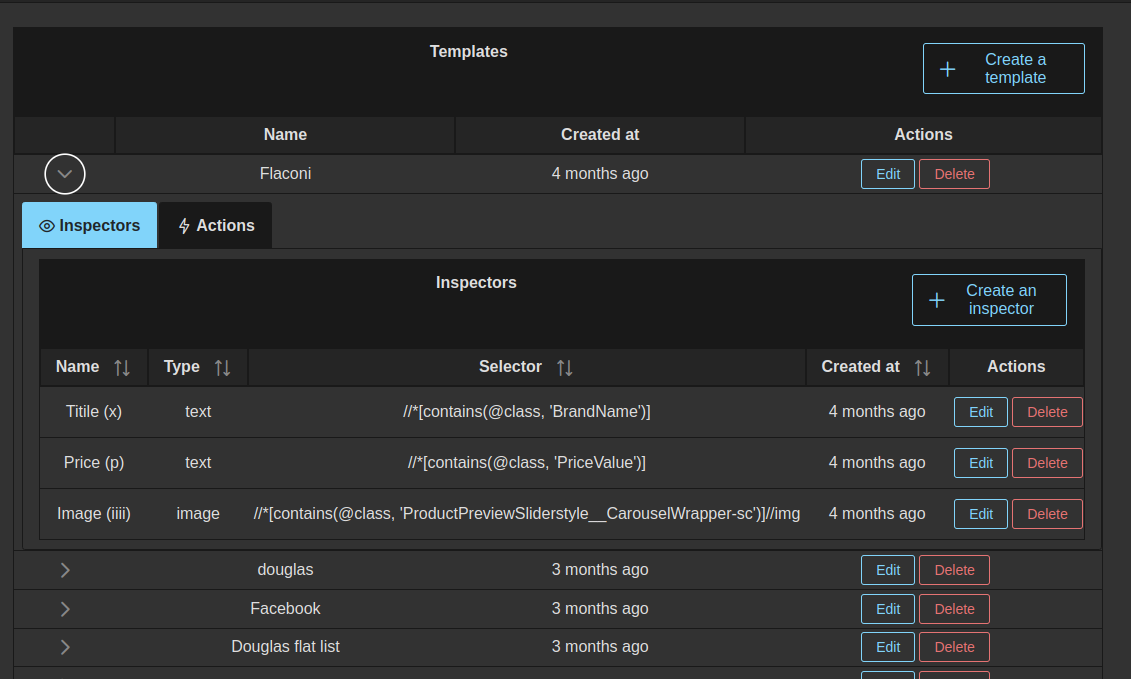
\includegraphics[width=13cm]{images/demo-3.png}
     \caption{High-level view of the software archtiticture.}
     \label{fig:software-arch}
\end{figure}

\begin{figure}[h]	
     \centering
     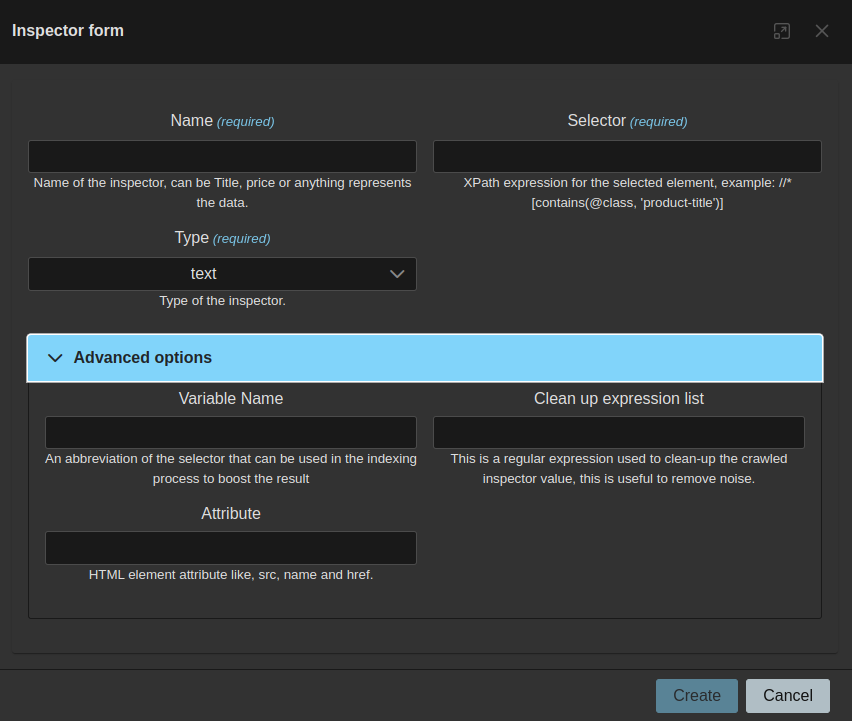
\includegraphics[width=13cm]{images/demo-4.png}
     \caption{High-level view of the software archtiticture.}
     \label{fig:software-arch}
\end{figure}

\begin{figure}[h]	
     \centering
     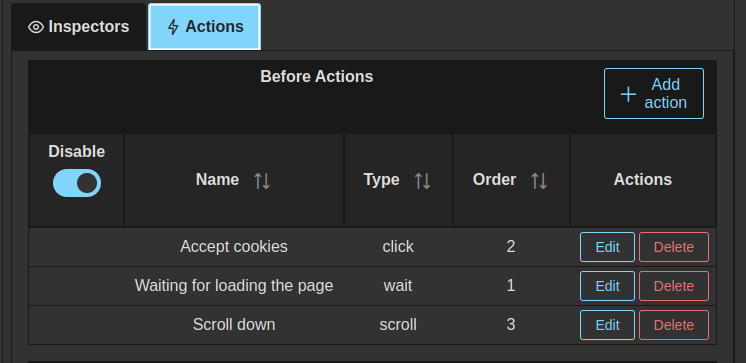
\includegraphics[width=13cm]{images/demo-5.png}
     \caption{High-level view of the software archtiticture.}
     \label{fig:software-arch}
\end{figure}

\begin{figure}[h]	
     \centering
     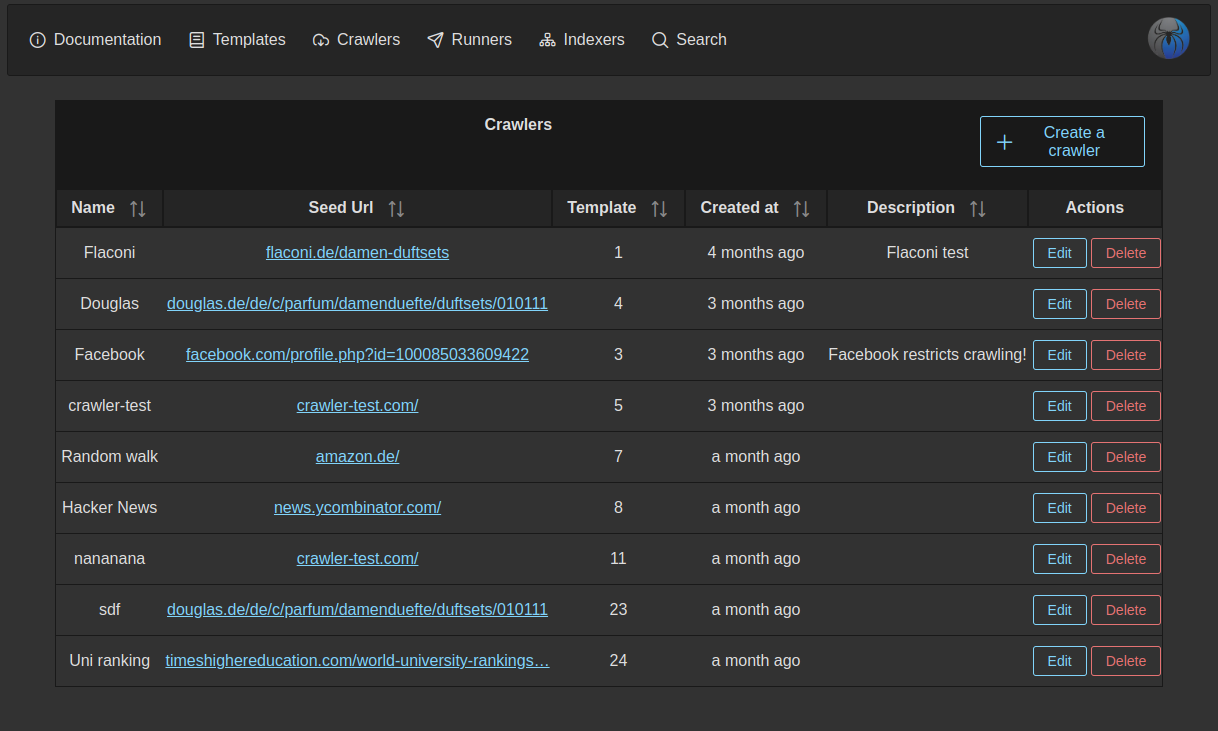
\includegraphics[width=13cm]{images/demo-6.png}
     \caption{High-level view of the software archtiticture.}
     \label{fig:software-arch}
\end{figure}

\begin{figure}[h]	
     \centering
     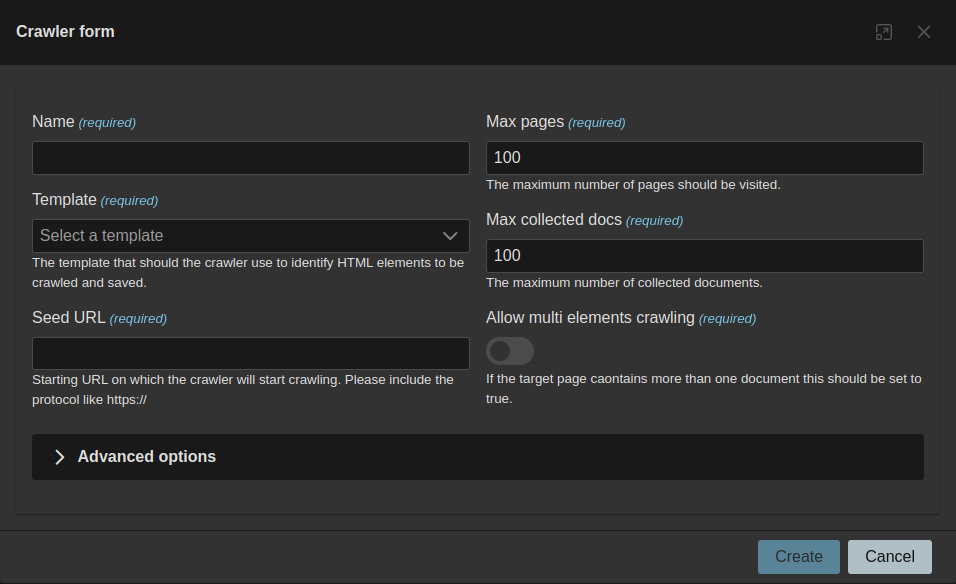
\includegraphics[width=13cm]{images/demo-7.png}
     \caption{High-level view of the software archtiticture.}
     \label{fig:software-arch}
\end{figure}

\begin{figure}[h]	
     \centering
     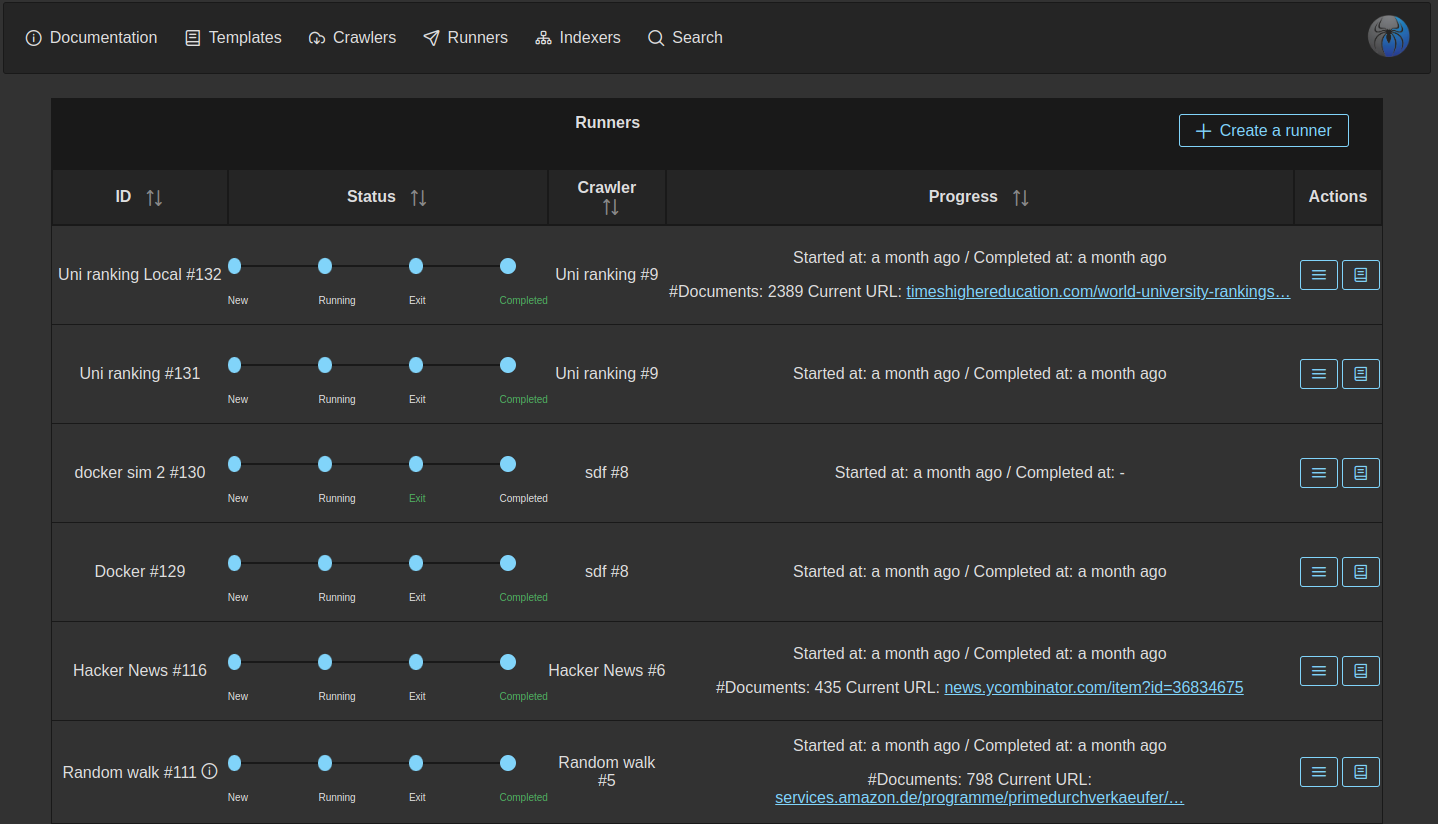
\includegraphics[width=13cm]{images/demo-8.png}
     \caption{High-level view of the software archtiticture.}
     \label{fig:software-arch}
\end{figure}

\begin{figure}[h]	
     \centering
     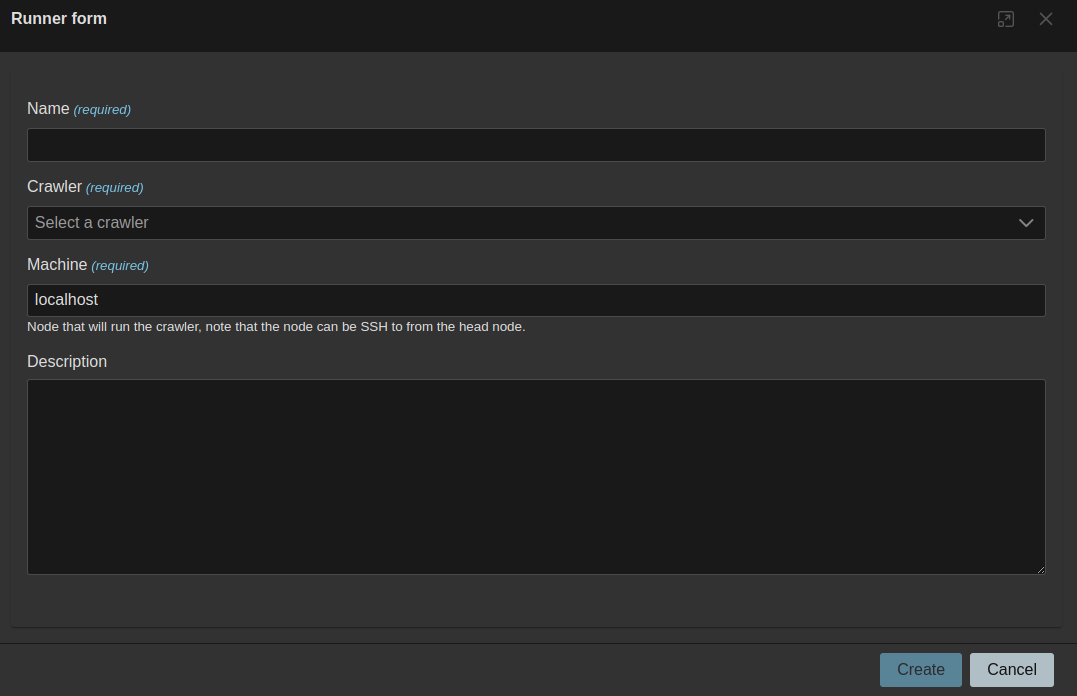
\includegraphics[width=13cm]{images/demo-9.png}
     \caption{High-level view of the software archtiticture.}
     \label{fig:software-arch}
\end{figure}

\begin{figure}[h]	
     \centering
     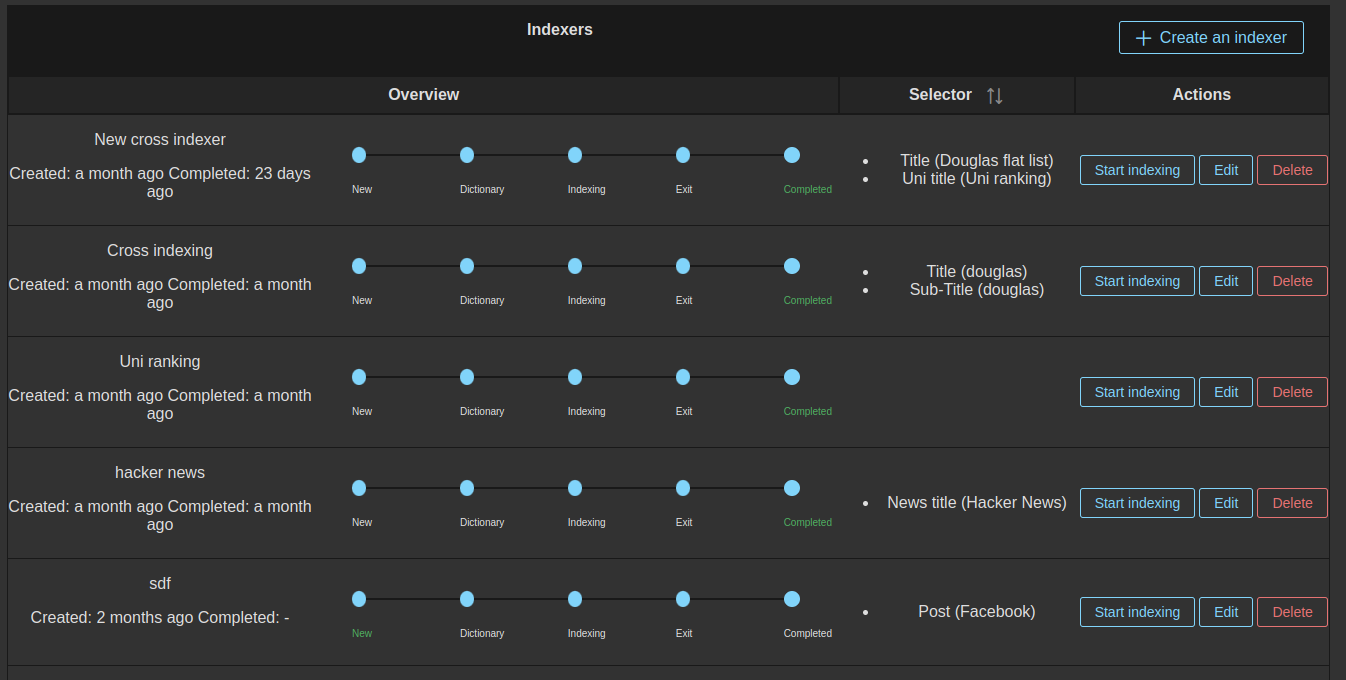
\includegraphics[width=13cm]{images/demo-10.png}
     \caption{High-level view of the software archtiticture.}
     \label{fig:software-arch}
\end{figure}

\begin{figure}[h]	
     \centering
     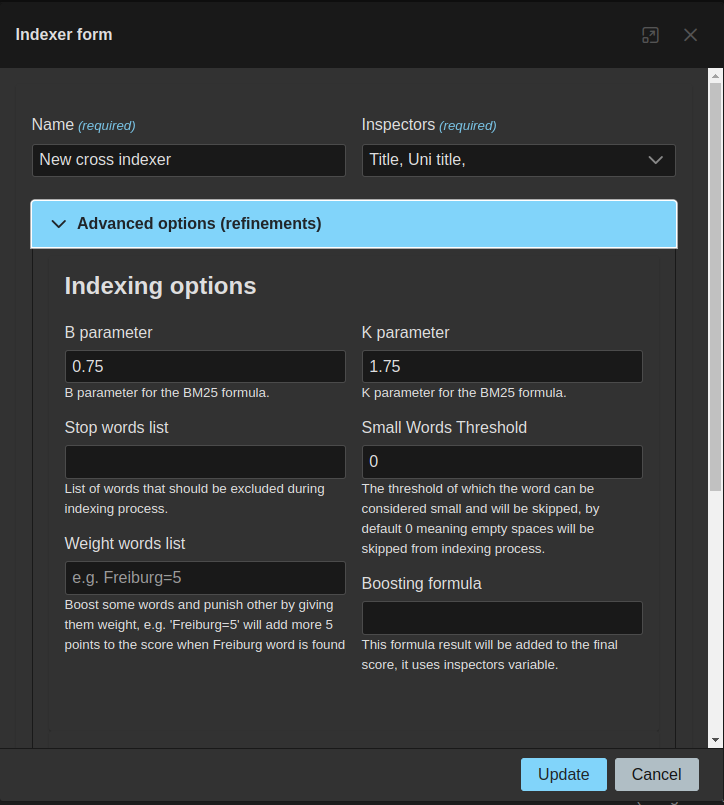
\includegraphics[width=13cm]{images/demo-11.png}
     \caption{High-level view of the software archtiticture.}
     \label{fig:software-arch}
\end{figure}

\begin{figure}[h]	
     \centering
     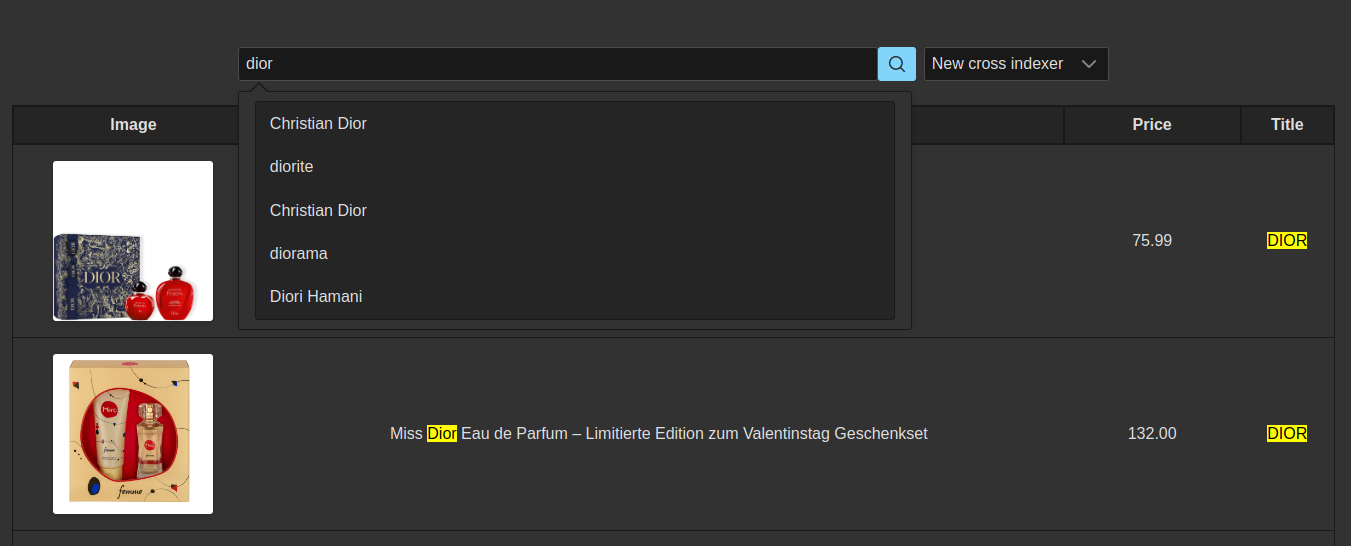
\includegraphics[width=13cm]{images/demo-12.png}
     \caption{High-level view of the software archtiticture.}
     \label{fig:software-arch}
\end{figure}